\Chapter{Koncepció}

A feladat fő problémája a háromszögek metszéspontjának kiszámítása a térben. Ez sajnos nem egy egyszerű feladat. Programozás terén, illetve erőforrásigény terén sem elhanyagolható.

A valóságban az emberi gondolkodásnak egyszerűnek tűnhet eldönteni, hogy két háromszög metszi-e egymást, vagy sem. Programozás, illetve matematika terén viszont sokkal nehezebb. Rengeteg számítást kell végeznünk ahhoz, hogy megbizonyosodjunk a háromszögek metszéséről.

\Section{Irodalomkutatás}
A metszéspontok számításhoz legmegfelelőbbnek \textbf{\href{https://www.geometrictools.com/Documentation/DynamicCollisionDetection.pdf}{David Eberly 1999-es kutatását}}, azon belül a \cite{triangles}(4.1 Separation of Triangles) szekciót találtam. A dokumentáció tökéletesen elmagyarázza a matematikai képletek elemeit, azok használatát, lépéseit. Ezek mind táblázatba szedve találhatóak. A pontos magyarázat a következő fejezetben található. Emellett rengeteg különböző módszer található az interneten térbeli modellek ütközésének vizsgálatához, például:\\
\newpage
\subsection{Négyzetes elválasztás:}
A négyzetes elválasztás módszere egy olyan algoritmus, amelyet számítógépes játékok, illetve számítógépi grafikában közkedvelten használnak ütközések érzékelésére.
A módszer segítségével meghatározhatjuk, hogy két vagy több modell metszik-e egymást vagy sem.
Az ötlet lényege, hogy minden modellt négyzet alakú "dobozokkal" vesszük körbe, amelyet a legkisebb négyszögű terület alapján határozzuk meg. Ekkor az ütközést csak akkor kell ellenőrizni, ha a meghatározott "dobozok" metszik egymást.\\
Lépései:
\begin{itemize}
\item Minden modellhez rendelünk egy "dobozt", amely a legkisebb területen határozza meg a modellt. Ez a "doboz" könnyen meghatározható 4 ponttal a térben.

\item Ellenőrizzük a "dobozokat", hogy metszik-e egymást vagy sem.

\item Ha két vagy több "doboz" metszik egymást, akkor kerül sor a pontos ütközésvizsgálatra (jelen szakdolgozat alapján ez háromszögek metszéspontjának számítása).
\end{itemize}
Előnye a módszernek, hogy a bonyolult modelleket leírhatjuk először egyszerű geomatria alakzattal, így az ütközésvizsgálat ideje nagyban csökken.\\
Hátránya a módszernek, hogy az algoritmus csak közelíti az eredményt, ezért fontos egyéb algoritmusokat alkalmazni a pontos ütközésvizsgálathoz.

\begin{figure}[h]
	\centering
	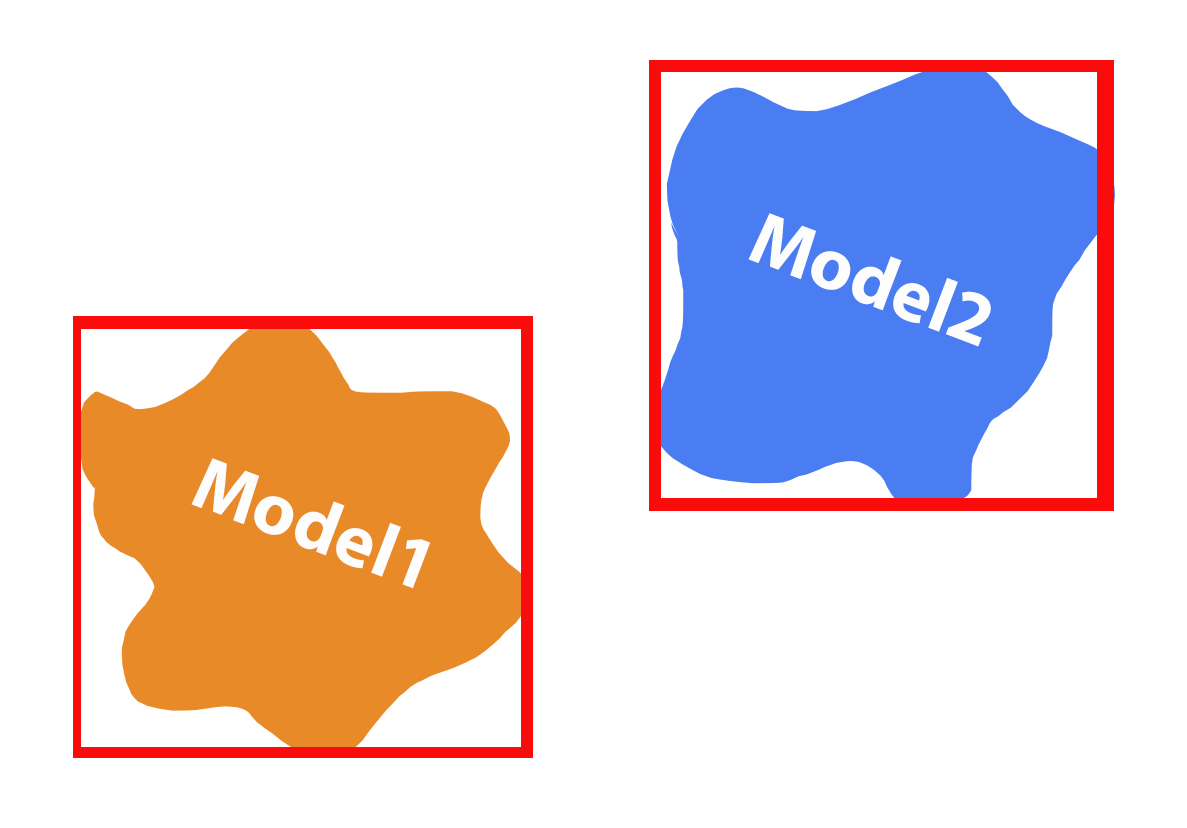
\includegraphics[width=13truecm, height=7.5truecm]{images/con1.png}
	\caption{Doboz rendelése modellekhez 2D-ben ábrázolva}
	\label{fig:con_1}
\end{figure}

\newpage

\subsection{Sugárkövetés módszere:}
A sugárkövetés módszere egy nagyon elterjedt technológia ütközések vizsgálatához. Ezzel a módszerrel valós időben tudjuk kiszámítani a világítást és az árnyékokat.
Az ötlet lényege, hogy a modellek és a fényforrások közötti interakciókat számítjuk. Egy sugarat bocsátunk ki a képpont irányába a kamera pozíciójából, és ellenőrizzük, hogy a sugár milyen modelleket metsz.
Így meg tudjuk határozni, hogy a képpont milyen modelltől kap fényt, illetve milyen árnyékokat, színeket szükséges megjeleníteni.
\\
Lépései:
\begin{itemize}
\item Létrehozzuk a sugarat minden képpontra a kamera pozíciójából. Így a sugár meghatározza a képpont irányát, illetve pozícióját.

\item Végighaladunk a sugár útján és ellenőrizzük milyen modellek metszik a sugarat.

\item Amikor a sugár metsz egy modellt, akkor kiszámítjuk az anyagtulajdonságokat. Például fényvisszaverődés, színek, tükröződés, árnyékolás.

\item A modellek és a fényforrások közti távolságok, illetve átlátszóságok alapján kiszámítjuk, hogy az adott pontba mennyi fény jut.

\item Néhány esetben továbbfejleszthető a módszer rekurzióval. Ez azt jelenti, hogy ha a sugár ütközik egy modellel, akkor további sugarakat hozunk létre. Ezzel részletesebb tükröződéseket hozhatunk létre.
\end{itemize}
Előnye a módszernek, hogy hatékonyan hozhatunk létre fotorealisztikus képeket.\\
Hátránya a módszernek, hogy a számítási igénye magas.

\begin{figure}[h]
	\centering
	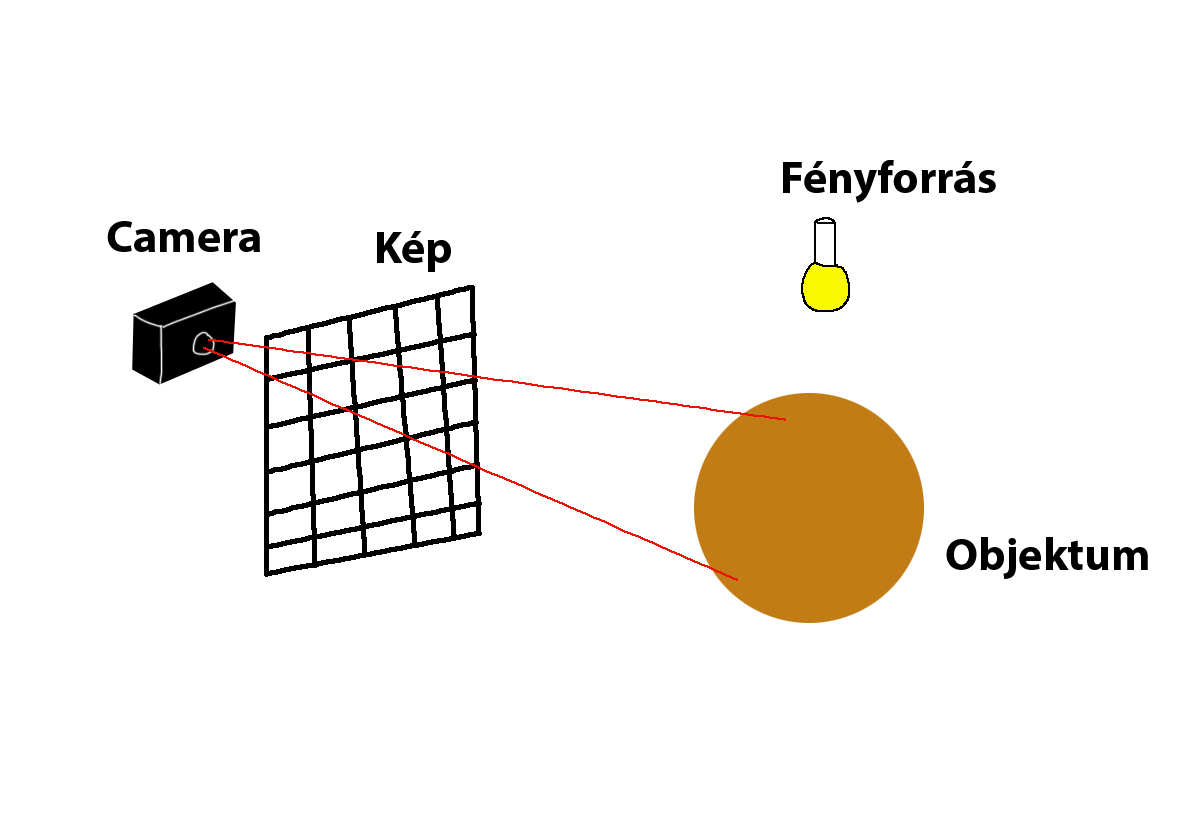
\includegraphics[width=13truecm, height=7.5truecm]{images/con2.png}
	\caption{Sugárkövetés alap gondolatának ábrázolása}
	\label{fig:con_2}
\end{figure}

\newpage
\subsection{Voxel-alapú:}
A voxel-alapú módszer egy hatékony módszer, amely a háromdimenziós teret felosztja kisebb részekre. A teret téglalap alakú részekre bontja, ezeket a részeket voxel-nek nevezzük.
Ezekkel a voxelekkel közelítjük a modelleket.
\\
Lépései:
\begin{itemize}
\item Voxel rácsot hozunk létre. Ezzel a ráccsal osztjuk fel a teret kisebb voxelekre. Ez egy háromdimenziós rács szerkezet.

\item A modelleket voxelekkel közelítjük, amelyek a voxel rácsban helyezkednek el. A pontosság módosítható a voxelek mérete alapján. Minden voxelt megjelöljük az alapján, hogy tartalmaz-e modellt vagy sem.

\item Ütközések vizsgálatához azt ellenőrizzük, hogy a két modellt tartalmazó voxel metszik-e egymást vagy sem. Ha egy aktív voxel metszi a másik aktív voxelt, akkor a modellek ütközhetnek egymással. Ezután szükséges egyéb ütközésvizsgálat a pontosításhoz.
\end{itemize}
Előnye a módszernek, hogy a használata egyszerű, a pontosság könnyen módosítható. Nagyobb tér esetén hatékony megoldás lehet. Az ütközésvizsgálat csak az aktív voxelek esetén történik meg, így elkerülhető a fölösleges számítások.\\
Hátránya a módszernek, hogy nehéz pontosan meghatározni a voxel rács méretét. Túl nagy méret esetén az ütközésvizsgálat nem lesz elég pontos, kis méret esetén a számítások költségesek lehetnek.
\begin{figure}[h]
	\centering
	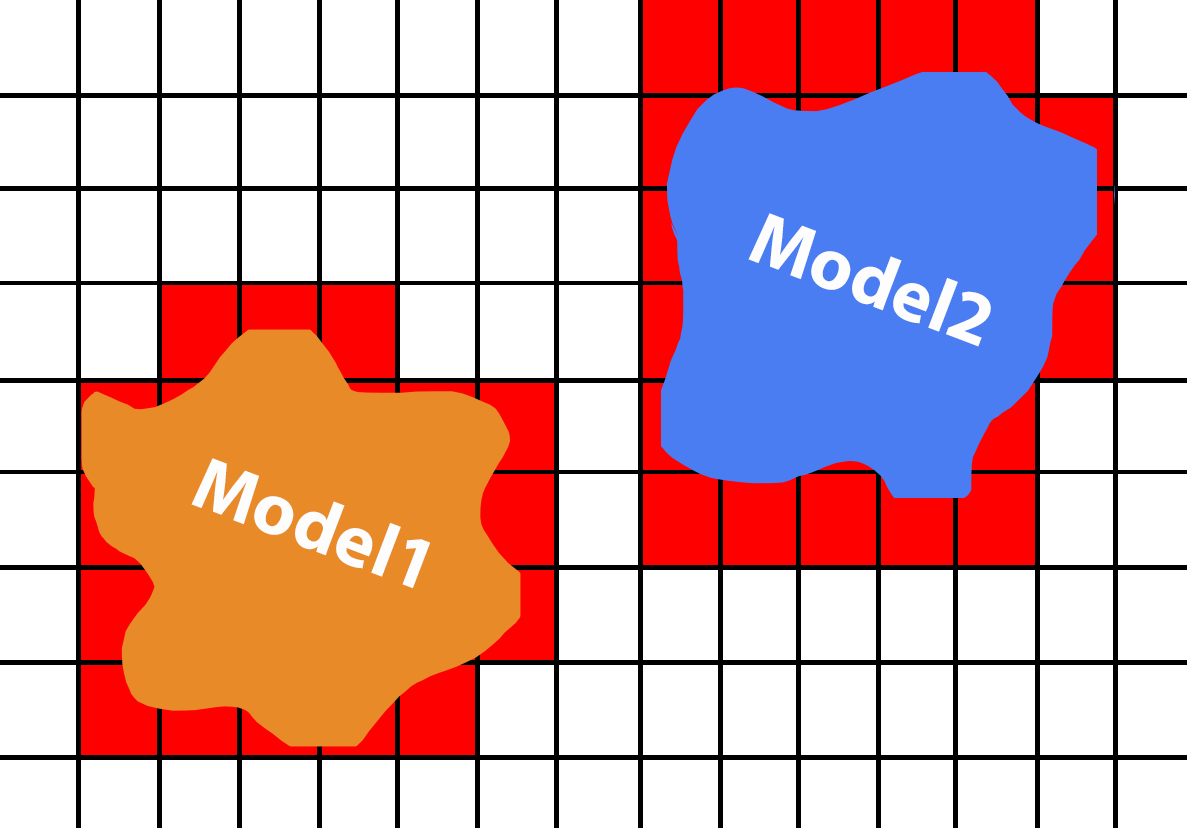
\includegraphics[width=13truecm, height=7.5truecm]{images/con3.png}
	\caption{A tér felbontása voxelekre 2 dimenzióban}
	\label{fig:con_3}
\end{figure}

\newpage
\subsection{Egyenletek alkalmazása:}
Az egyenletek alkalmazásának módszere egy elterjedt technológia. A módszer alapötlete, hogy matematikai egyenletek segítségével határozza meg a modellek mozgásának, illetve ütközéseinek érzékelésére.
\\
Lépései:
\begin{itemize}
\item Felállítunk egy matematikai modellt, amely leírja a modellek mozgását.

\item Definiáljuk az ütközések vizsgálatához szükséges szabályokat, feltételeket. Ezek a feltételek lehetnek egyszerűbbek, vagy komplexebbek, például távolságok, sebességek, fizikai tulajdonságok, formák, méretek.

\item A meghatározott modell és a feltételek alapján ellenőrizzük az ütközésvizsgálatot.\

\item Gyakran szükség van az egyenletek alkalmazására numerikus módszerekre, például differenciálegyenletek megoldása esetén.
\end{itemize}
Előnye a módszernek, hogy pontos fizikai szimulációkat érzékelhetünk.\\
Hátránya a módszernek, hogy magas a számítási igénye, ezért nem alkalmas valós idejű szimulációkra, illetve magas modellszám esetén sem előnyös.